\section{METODOLOGI}

\subsection{Desain Robot yang Digunakan}

\begin{figure} [ht] \centering
	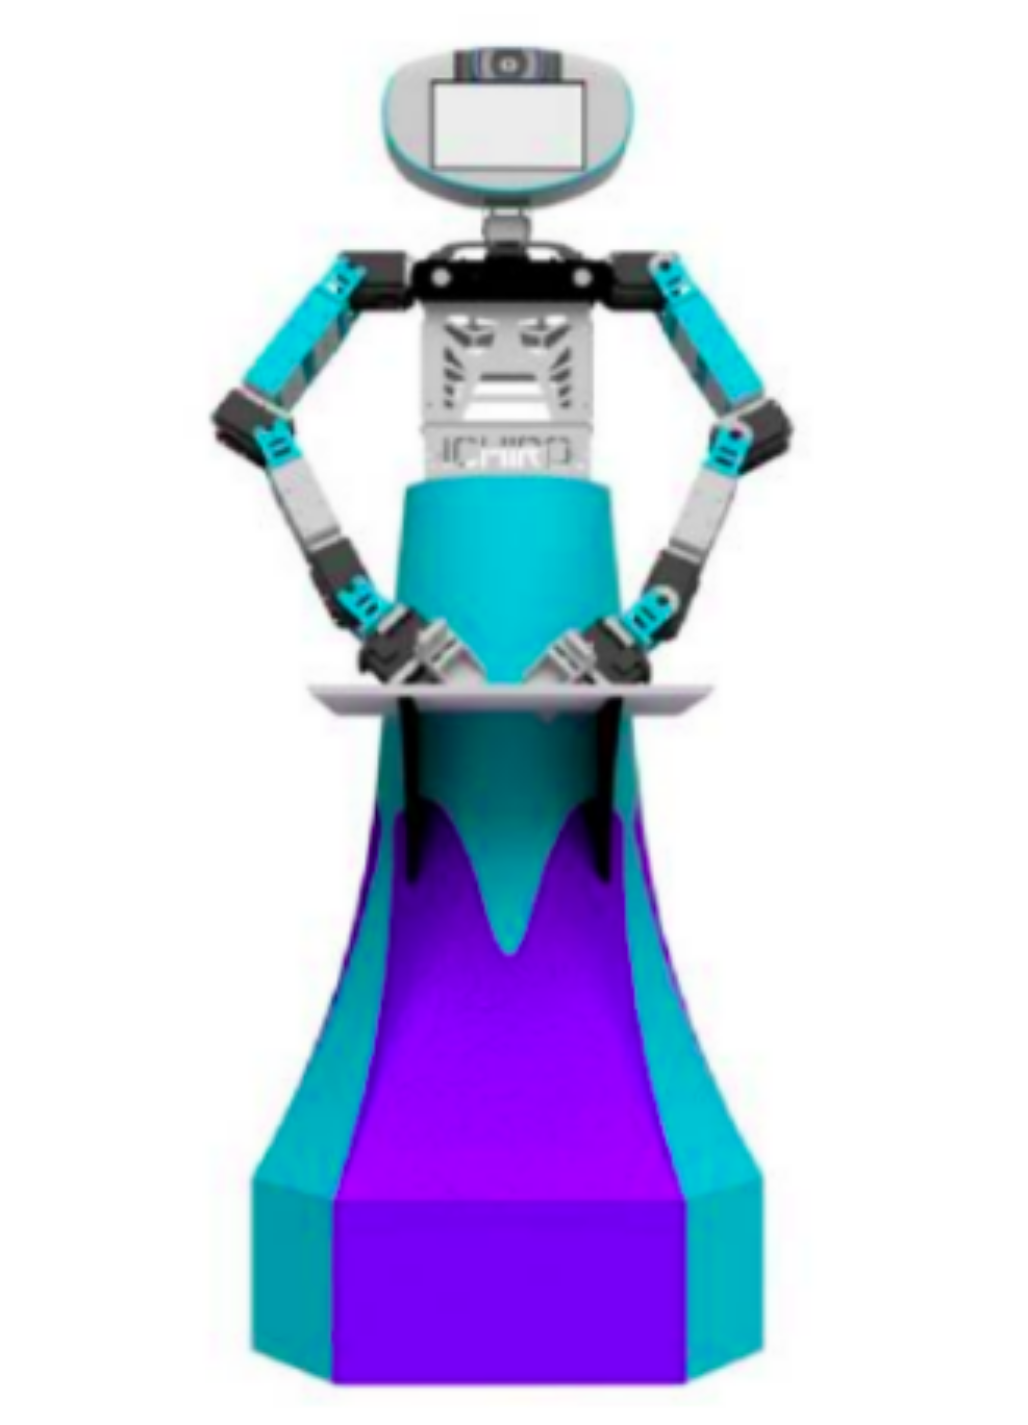
\includegraphics[scale=0.45]{gambar/robot-design.png}
	\caption{Desain Robot yang Digunakan}
	\label{fig:RobotDesign}
\end{figure}

Robot yang akan digunakan pada pada penelitian ini memiliki desain \emph{mobile humanoid robot} \citep{Mohamed2012}, yang merupakan gabungan antara robot mobile dan robot humanoid.
Seperti yang terlihat pada gambar \ref{fig:RobotDesign}, bagian bawah robot menyerupai robot mobile dengan \emph{differential wheels} yang memungkinkan pergerakan ke segala arah secara dua dimensi, sedangkan bagian atas robot menyerupai robot humanoid yang terdiri atas badan, kepala, dan lengan.
Dengan desain mobile humanoid robot ini, diharapkan pengguna bisa merasakan interaksi sosial yang lebih baik dengan robot karena memiliki bentuk mendekati manusia \citep{Rossi2018} sambil mempermudah navigasi dari robot ke berbagai tempat.

Robot ini dilengkapi dengan beberapa sensor seperti IMU (\emph{inertial measurement unit}) untuk mengetahui orientasi dari robot dan sensor kamera di kepala untuk mendeteksi objek menggunakan visi komputer.
Selain itu robot ini juga dilengkapi dengan dua lengan seperti robot manipulator yang bisa diatur pada berbagai posisi dan orientasi \citep{Iqbal2012}.
Dengan adanya sensor dan lengan ini diharapkan robot mampu melakukan tindakan assistive secara sosial sesuai dengan data yang didapatkan dari sensor yang ada.

\subsection{Pengembangan Controller Robot}

\begin{figure} [ht] \centering
	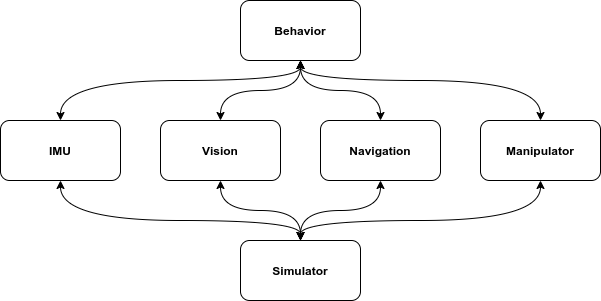
\includegraphics[scale=0.45]{gambar/robot-controller.png}
	\caption{Diagram sistem controller robot}
	\label{fig:RobotController}
\end{figure}

Controller robot yang digunakan untuk simulasi akan dikembangkan menggunakan ROS 2.
Controller tersebut akan dipisah menjadi beberapa node seperti yang terlihat pada gambar \ref{fig:RobotController}.
Setiap node yang ada akan terhubung satu sama lain menggunakan sistem komunikasi antar proses ROS 2 yang berupa topics dan services.

Bagian utama dari controller robot tersebut adalah node Behavior yang berisi program yang mengatur segala tindakan robot berdasarkan data yang didapat dari sensor yang ada di simulasi.
Kemudian node Behavior tersebut akan terhubung dengan empat node lain yang merepresentasikan sensor dan aktuator yang ada pada robot.
Keempat node tersebut adalah node IMU yang akan memproses data dari sensor IMU yang ada di robot, node Vision yang akan memproses program visi komputer menggunakan gambar yang didapat dari kamera robot, node Navigation yang mengatur pergerakan robot, dan node Manipulator yang mengatur posisi dan orientasi dari lengan robot.
Terakhir, keempat node sensor dan aktuator tersebut akan terhubung dengan node Simulator, yang dalam hal ini adalah simulator Gazebo.

\subsection{Pembuatan Lingkungan Simulasi}

Lingkungan simulasi dibuat menggunakan \emph{Gazebo}.

\subsection{Pengujian Sistem Robot terhadap Lingkungan Simulasi}

Pengujian sistem robot akan dilakukan untuk setiap fungsionalitas yang dimiliki robot.
